\section{Methodology}
\subsection{Dataset}
The dataset used in this assignment was provided by the instructor. It consists of a set of instances, each labeled as either normal or anomalous. The specific details of the dataset, such as the number of features and the distribution of normal and anomalous instances, were not disclosed.

Figure \ref{fig:nominal_train} shows a random selection of 16 nominal images from the training set, while Figure \ref{fig:anomaly_train} displays a random selection of 16 anomalous images from the training set. Similarly, Figure \ref{fig:nominal_test} and Figure \ref{fig:anomaly_test} present random selections of nominal and anomalous images from the test set, respectively.

\begin{figure}[htbp]
\centering
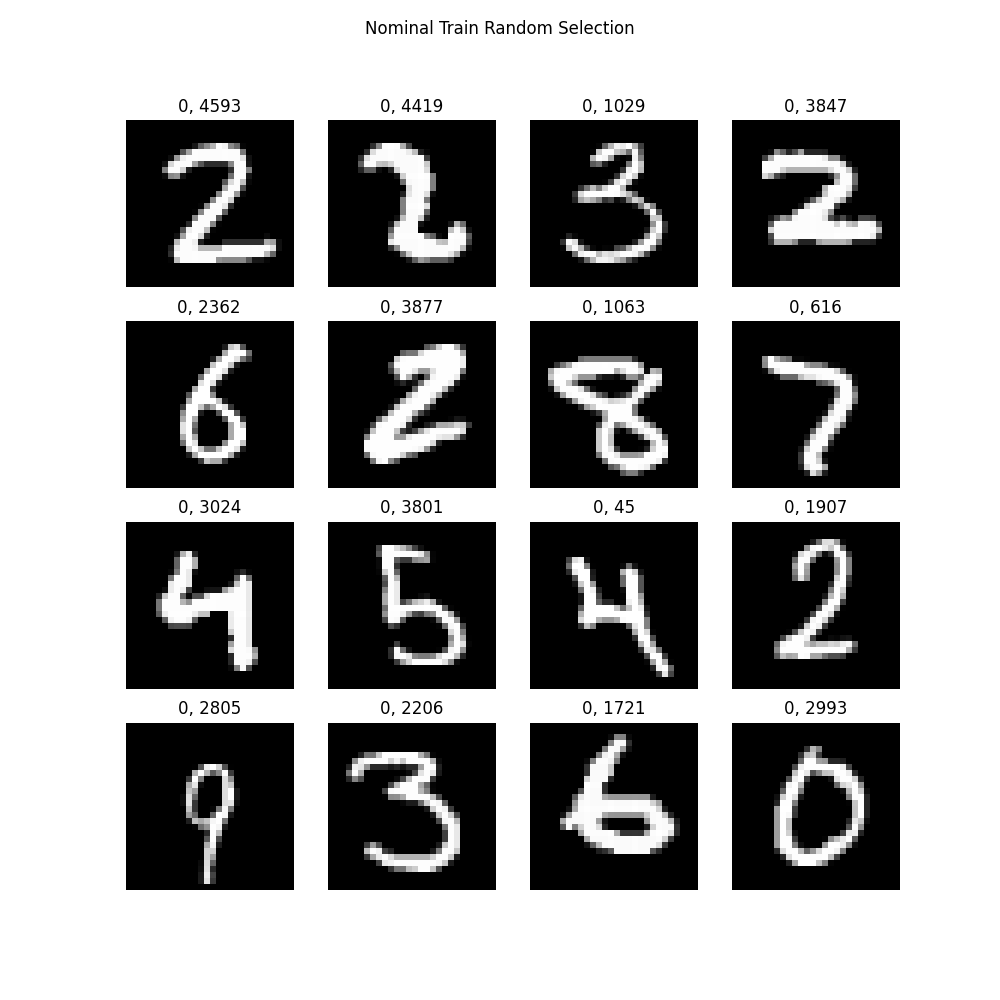
\includegraphics[width=0.5\textwidth]{resources/images/_nominal_train_random_selection.png}
\caption{Random selection of nominal images from the training set}
\label{fig:nominal_train}
\end{figure}

\begin{figure}[htbp]
\centering
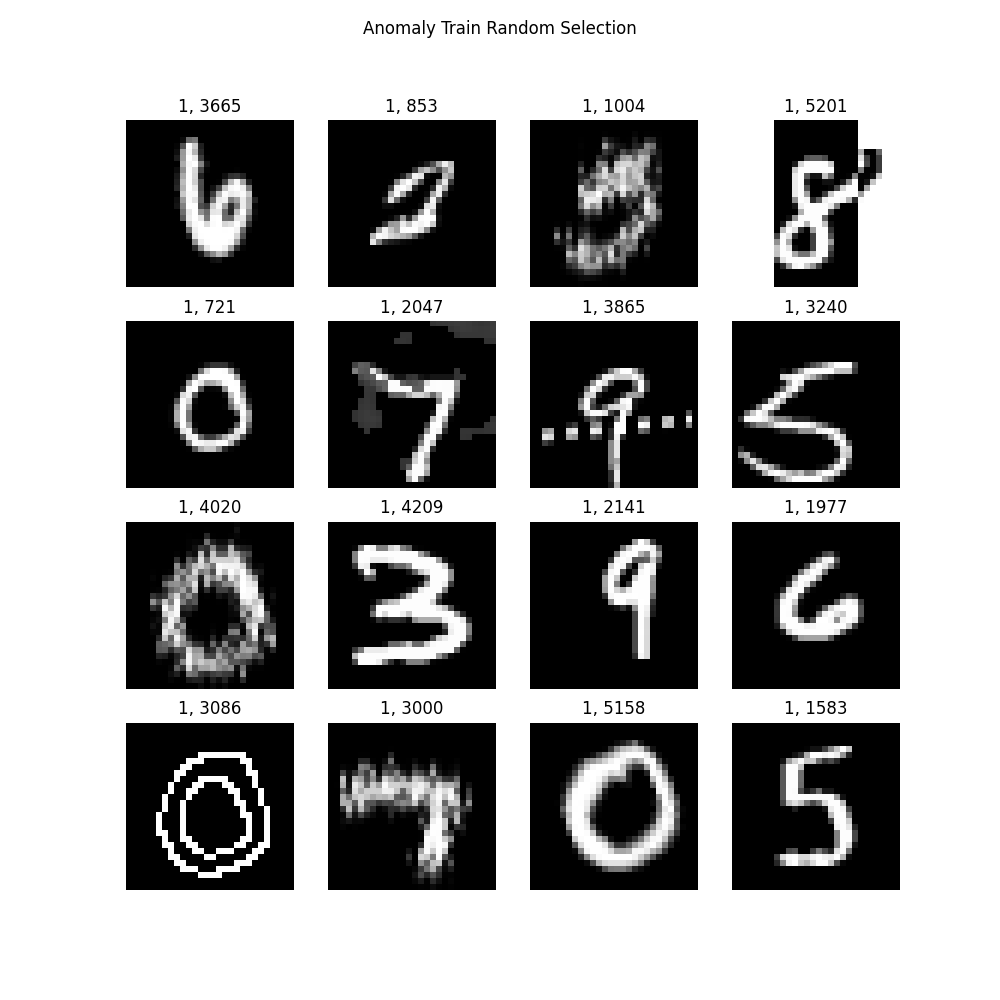
\includegraphics[width=0.5\textwidth]{resources/images/_anomaly_train_random_selection.png}
\caption{Random selection of anomalous images from the training set}
\label{fig:anomaly_train}
\end{figure}

\begin{figure}[htbp]
\centering
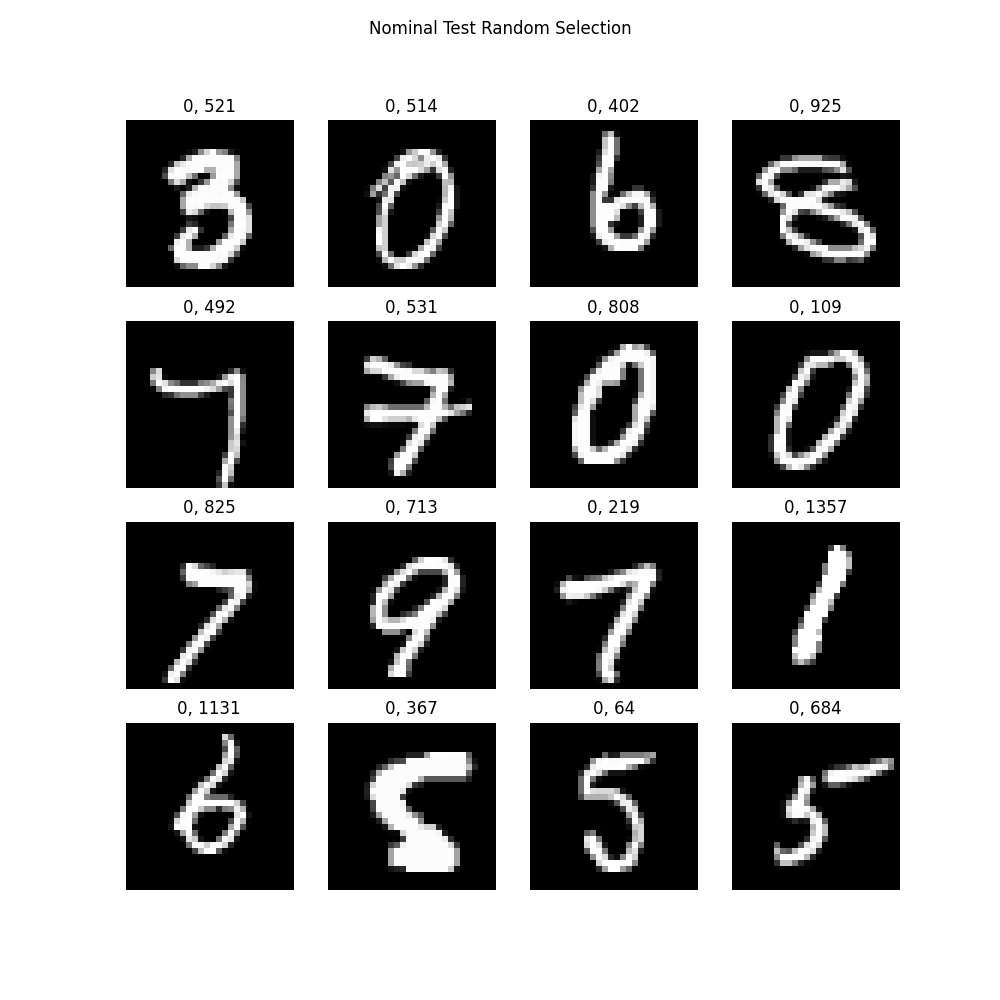
\includegraphics[width=0.5\textwidth]{resources/images/_nominal_test_random_selection.png}
\caption{Random selection of nominal images from the test set}
\label{fig:nominal_test}
\end{figure}

\begin{figure}[htbp]
\centering
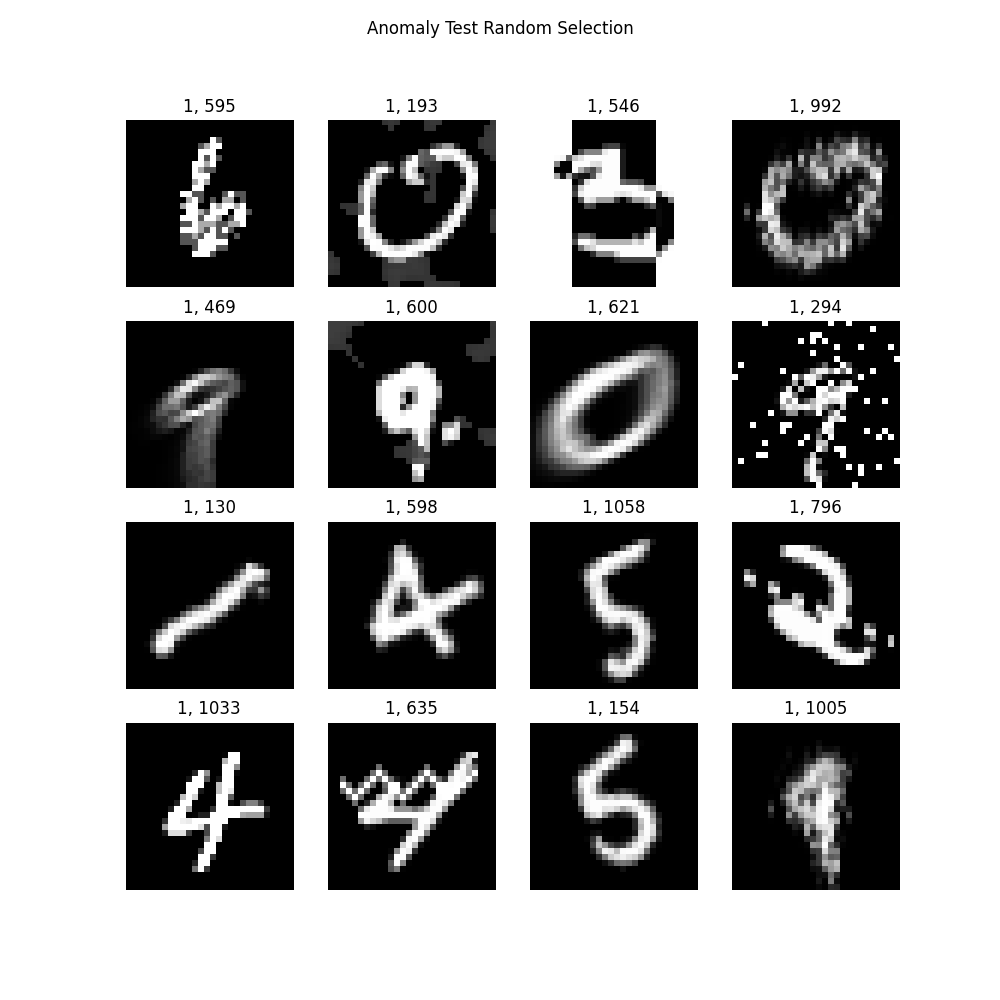
\includegraphics[width=0.5\textwidth]{resources/images/_anomaly_test_random_selection.png}
\caption{Random selection of anomalous images from the test set}
\label{fig:anomaly_test}
\end{figure}

\subsection{Isolation Forest Implementation}
We implement the Isolation Forest algorithm from scratch using Python. The algorithm consists of two main components: Isolation Tree (iTree) and Isolation Forest (iForest).

An iTree is a binary tree structure that recursively partitions the data based on randomly selected features and split points until instances are isolated or a maximum tree height is reached. The key idea is that anomalies require fewer partitions on average to be isolated compared to normal instances.

The iForest is an ensemble of iTrees. It constructs multiple iTrees using subsamples of the training data and aggregates the anomaly scores obtained from each iTree to make the final prediction.

The anomaly score of an instance is calculated based on the average path length it takes to be isolated in the iForest. Anomalies tend to have shorter average path lengths compared to normal instances.

\subsection{Evaluation Metrics}
To evaluate the performance of the Isolation Forest algorithm, we use the area under the Receiver Operating Characteristic (ROC) curve and the Precision-Recall (PR) curve. The ROC curve plots the true positive rate against the false positive rate at various threshold settings, while the PR curve plots precision against recall. Higher areas under these curves indicate better anomaly detection performance.